\documentclass{article}


\usepackage[utf8]{inputenc}
\usepackage{longtable}
\usepackage{authblk}
\usepackage{adjustbox}

\usepackage{natbib}

\title{IDH EN COLOMBIA}
% autores

\author[1]{\normalsize Giancarlo Melani Hurtado}


\affil[1,2]{\small  Departamento de Ingenieria,Universidad de los Andes\\
\texttt{{g.melani10}@uniandes.edu.col}}
\affil[1]{\small Curso de verano, herramientas computacionales\\
Uniandes\\
\texttt{delcurso@bp.com.col}}

\date{29 de Junio de 2018}

%%%
\usepackage{Sweave}
\begin{document}
\Sconcordance{concordance:ProyectoIntegrador.tex:ProyectoIntegrador.Rnw:%
1 25 1 1 0 26 1 1 5 1 1 1 5 15 0 1 2 3 1 1 6 1 2 6 1 1 8 1 2 10 1 1 4 %
12 0 1 2 3 1 1 9 13 0 1 2 3 1 1 3 1 2 9 1 1 5 1 4 31 0 1 2 8 1 1 14 1 %
17 1 1 1 14 1 3 10 1}



\maketitle


\begin{abstract}
Este es un trabajo que busca generar un paper a traves del uso de la herramienta Latex para le ejecucion de un PDF que permita generar un archivo comprensible y amigable. Por otra parte se usa Python para realizar la limpieza de los datos que se usan para los analisis y de R-Studio para generar el documento.

\end{abstract}

\section*{Introduccion}

El seguiente paper corresponde al proyecto integrador del curso herramientas computacionales en el que se tratara el tema del indice de desarrollo humano (IDH).Este es un indicador que elabora cada ano Naciones Unidas. Se trata de un indicador que, a diferencia de los que se utilizaban anteriormente que median el desarrollo economico de un pais, analiza la salud, la educacion y los ingresos.
Si ordenamos los paises en funcion de su indice de desarrollo humano, Colombia se encuentra en el puesto 95 del ranking de desarrollo humano(IDH). El IDH, tiene en cuenta tres variables: vida larga y saludable, conocimientos y nivel de vida digno. Por lo tanto, influyen entre otros el hecho de que la esperanza de vida en Colombia estan en 74,2 anos, su tasa de mortalidad en el 5,94 y su renta per capita sea de 5.451 euros.

Comencemos viendo que hay en la sección \ref{univariada} en la página \pageref{univariada}.

\clearpage

\section{Exploración Univariada}\label{univariada}

Se denomina exploracion univariada al proceso en el que se obtiene las medidas estadisticas, la tabla de frecuencias y algun grafico de resumen de una variable en particular. Primero es necesario identificar la escala en la que esta medida la variable. Una clasificacion ampliamente usada es la que identifica tres tipos de variables: categoricas nominales, categoricas ordinales y numericas o escalares. Las categoricas pueden clasificarse a su vez por la cantidad de categorias o modalidades que puedan tener: dicotomicas o politomicas. Reconocidas las variables es necesario saber que medidas y graficas corresponden o se pueden obtener. Una nominal no puede tener media ni mediana, solo moda. Una ordinal puede tener moda y mediana pero no media. Una numerica puede tener las tres: moda, mediana y media. A estas medidas se les reconoce como medidas representativas de la variable o medidas de centralidad.Esto lo menciona Macqueen en sus libros.\cite{macqueen_methods_nodate}





% Table created by stargazer v.5.2.2 by Marek Hlavac, Harvard University. E-mail: hlavac at fas.harvard.edu
% Date and time: vie., jun. 29, 2018 - 8:18:00 p. m.
\begin{table}[!htbp] \centering 
  \caption{Medidas estadisticas} 
  \label{stats} 
\begin{tabular}{@{\extracolsep{5pt}}lcc} 
\\[-1.8ex]\hline 
\hline \\[-1.8ex] 
Statistic & \multicolumn{1}{c}{N} & \multicolumn{1}{c}{Median} \\ 
\hline \\[-1.8ex] 
IDH & 32 & 0.804 \\ 
Población.Cabecera & 32 & 717,197 \\ 
Población.Resto & 32 & 268,111.5 \\ 
Población.Total & 32 & 1,028,429 \\ 
\hline \\[-1.8ex] 
\end{tabular} 
\end{table} 
Se procedio a realizar un analisis estadistico de los datos, motivo por el cual se comenzo con unos histogramas como se evidencia a continuacion:

\begin{figure}[h]
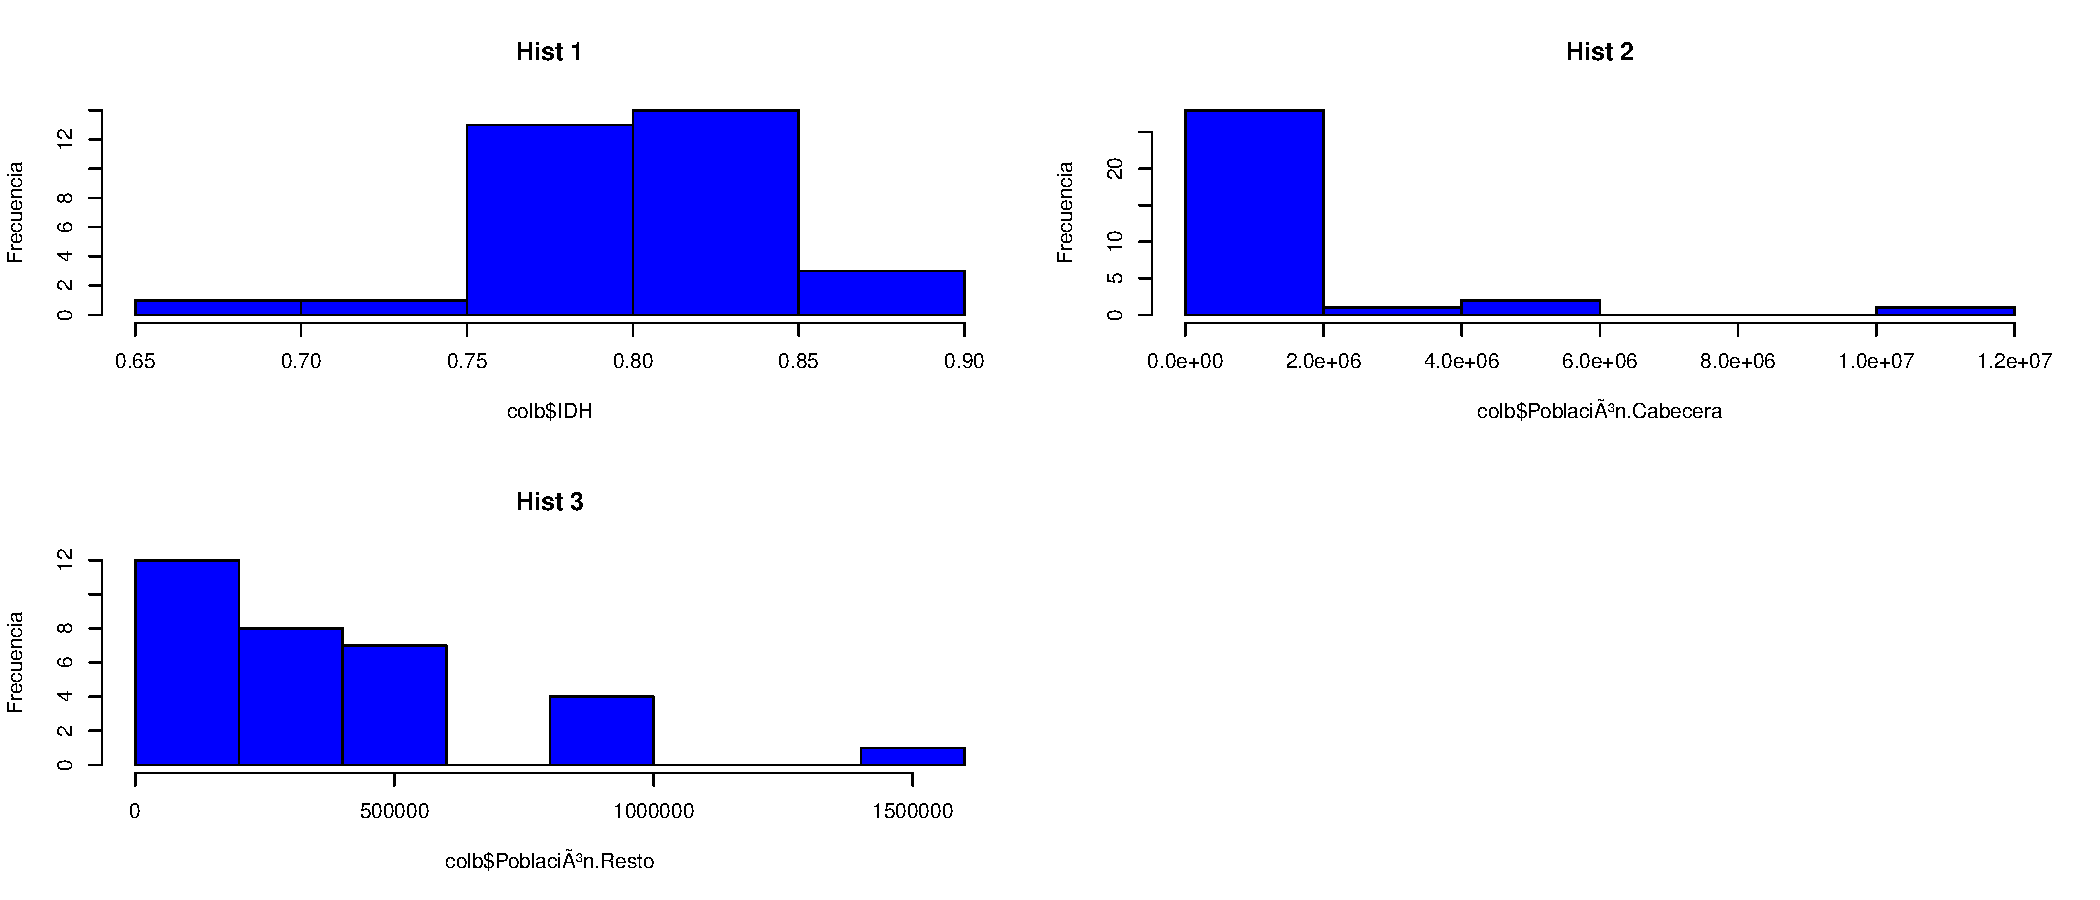
\includegraphics{ProyectoIntegrador-hist}
\caption{Histogramas }
\end{figure}
 
 A continuacion, se presentan los histogramas luego de realizar las transformaciones.


\begin{figure}[h]
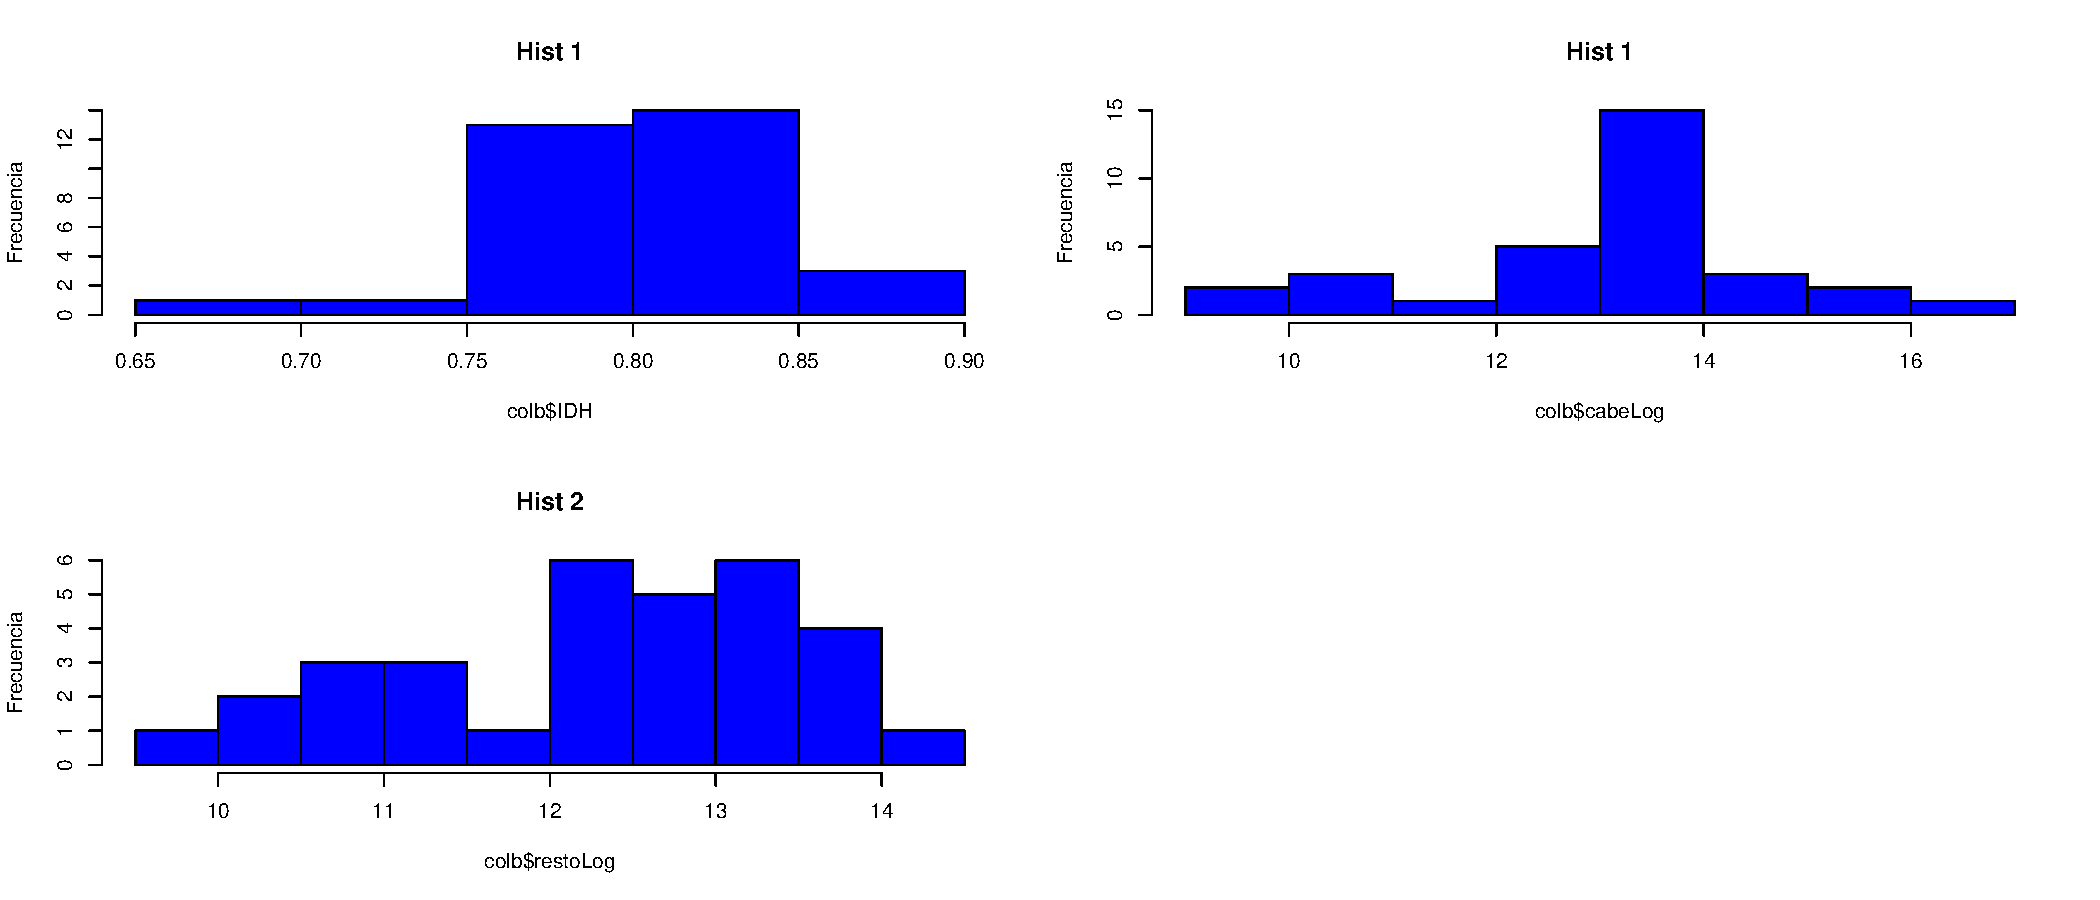
\includegraphics{ProyectoIntegrador-log}
\caption{Histogramas luego de la transformación}
\end{figure}

\clearpage


\section{Exploración Bivariada}


En este trabajo estamos interesados en el impacto de los otros indices. Veamos las relaciones bivariadas que tiene esta variable con todas las demás:

% Table created by stargazer v.5.2.2 by Marek Hlavac, Harvard University. E-mail: hlavac at fas.harvard.edu
% Date and time: vie., jun. 29, 2018 - 8:18:17 p. m.
\begin{table}[!htbp] \centering 
  \caption{Correlacion de IDH con las demás variables} 
  \label{corrDem} 
\begin{tabular}{@{\extracolsep{5pt}} cc} 
\\[-1.8ex]\hline 
\hline \\[-1.8ex] 
cabeLog & restoLog \\ 
\hline \\[-1.8ex] 
$0.487$ & $0.177$ \\ 
\hline \\[-1.8ex] 
\end{tabular} 
\end{table} 

Veamos la correlacionn entre las variables independientes:

% Table created by stargazer v.5.2.2 by Marek Hlavac, Harvard University. E-mail: hlavac at fas.harvard.edu
% Date and time: vie., jun. 29, 2018 - 8:18:17 p. m.
\begin{table}[!htbp] \centering 
  \caption{Correlacion entre variables independientes} 
  \label{corrTableX} 
\begin{tabular}{@{\extracolsep{5pt}} ccc} 
\\[-1.8ex]\hline 
\hline \\[-1.8ex] 
 & cabeLog & restoLog \\ 
\hline \\[-1.8ex] 
cabeLog & 1 &  \\ 
restoLog & 0.84 & 1 \\ 
\hline \\[-1.8ex] 
\end{tabular} 
\end{table} 


\begin{figure}[h]
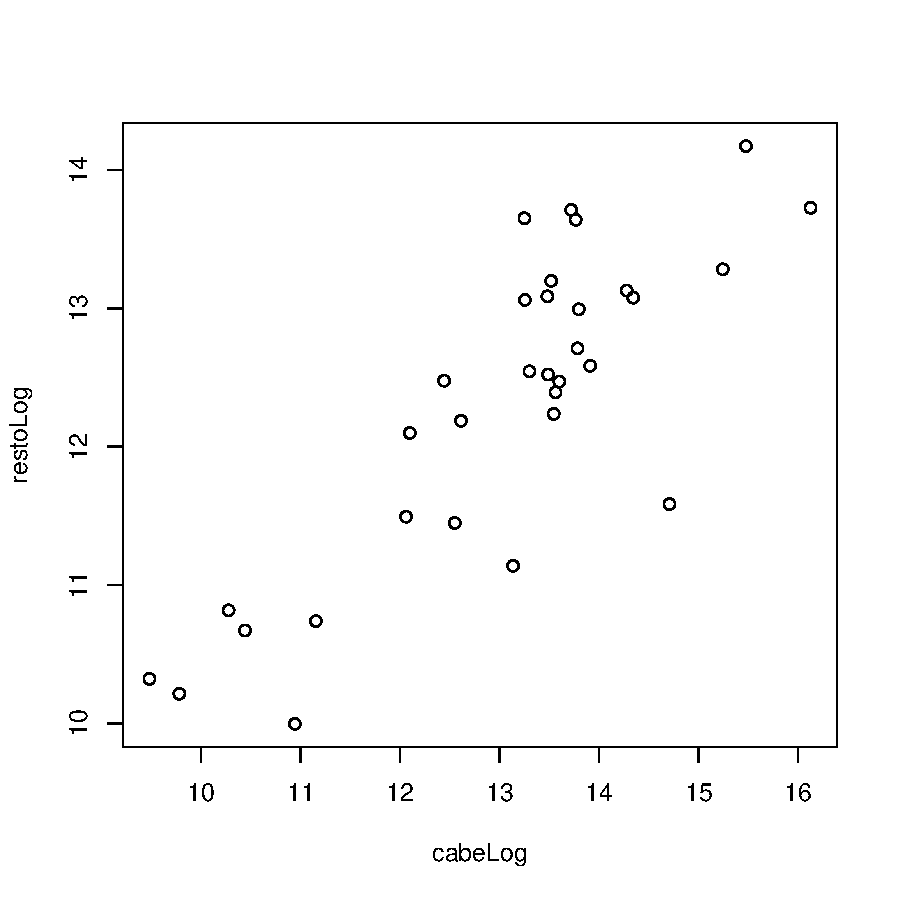
\includegraphics{ProyectoIntegrador-grafico}
\caption{Grafico de dispersion}
\end{figure}

\clearpage


\section{Modelos de Regresion}

En estadIstica, el analisis de la regresion es un proceso estadistico para estimar las relaciones entre variables. Incluye muchas tecnicas para el modelado y analisis de diversas variables, cuando la atencion se centra en la relación entre una variable dependiente y una o mas variables independientes (o predictoras).


% Table created by stargazer v.5.2.2 by Marek Hlavac, Harvard University. E-mail: hlavac at fas.harvard.edu
% Date and time: vie., jun. 29, 2018 - 8:18:18 p. m.
\begin{table}[!htbp] \centering 
  \caption{Modelos de Regresion} 
  \label{regresiones} 
\begin{tabular}{@{\extracolsep{5pt}}lcc} 
\\[-1.8ex]\hline 
\hline \\[-1.8ex] 
 & \multicolumn{2}{c}{\textit{Dependent variable:}} \\ 
\cline{2-3} 
\\[-1.8ex] & \multicolumn{2}{c}{IDH} \\ 
\\[-1.8ex] & (1) & (2)\\ 
\hline \\[-1.8ex] 
 cabeLog & 0.013$^{***}$ & 0.031$^{***}$ \\ 
  & (0.004) & (0.007) \\ 
  & & \\ 
 restoLog &  & $-$0.030$^{***}$ \\ 
  &  & (0.010) \\ 
  & & \\ 
 Constant & 0.634$^{***}$ & 0.766$^{***}$ \\ 
  & (0.055) & (0.065) \\ 
  & & \\ 
\hline \\[-1.8ex] 
Observations & 32 & 32 \\ 
R$^{2}$ & 0.238 & 0.425 \\ 
Adjusted R$^{2}$ & 0.212 & 0.385 \\ 
Residual Std. Error & 0.037 (df = 30) & 0.033 (df = 29) \\ 
F Statistic & 9.347$^{***}$ (df = 1; 30) & 10.706$^{***}$ (df = 2; 29) \\ 
\hline 
\hline \\[-1.8ex] 
\textit{Note:}  & \multicolumn{2}{r}{$^{*}$p$<$0.1; $^{**}$p$<$0.05; $^{***}$p$<$0.01} \\ 
\end{tabular} 
\end{table} 
\clearpage


\section{Exploracion Espacial}

La exploracion espacial designa los esfuerzos del ser humano en estudiar el espacio y sus astros desde el punto de vista cientifico y de su explotacion economica. Estos esfuerzos pueden involucrar tanto seres humanos viajando en naves espaciales como satelites con recursos de telemetria o sondas teleguiadas enviadas a otros planetas (orbitando o aterrizando en la superficie de estos cuerpos celestes). La ciencia que estudia los vuelos espaciales y la tecnologia relacionada con ellos se denomina astronautica. Las personas que pilotan naves espaciales, o son pasajeros en ellas, se llaman astronautas (en Rusia: cosmonautas; en China: taikonautas). Tecnicamente se considera astronauta a todo aquel que emprenda un vuelo suborbital (sin entrar en orbita) u orbital a como minimo 100 km de altitud (considerado el limite externo de la atmosfera).

\begin{figure}[h]



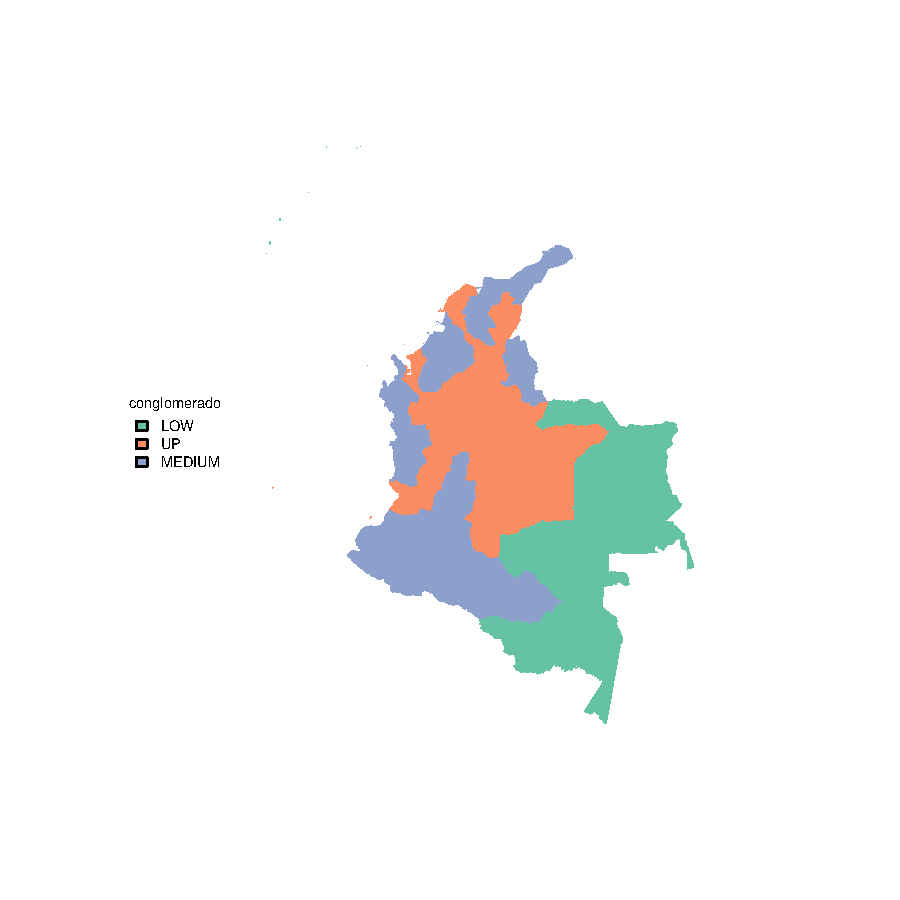
\includegraphics{ProyectoIntegrador-plotMap1}
\caption{Mapa de Colombia por colores}
\end{figure}

\clearpage

\bibliographystyle{abbrv}
\renewcommand{\refname}{Bibliografia}
\bibliography{PROYECTOZ}


\end{document}
